\section{Data Mining}
\label{section:mining}

\begin{wrapfigure}{r}{0.4\textwidth}
\vspace{-1.2cm}
\begin{center}
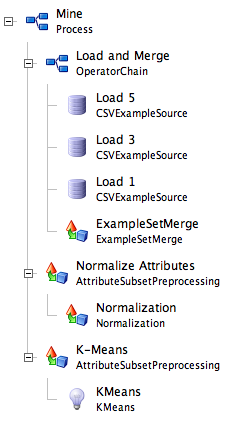
\includegraphics[scale=0.7]{images/mine.png}
\end{center}
\caption{Mine Process}
\label{figure:mine}
\end{wrapfigure}

Since all the data coming from the preprocessing are unlabeled, we chose an unsupervised learning approach for our mining process which is shown in Figure \ref{figure:mine}; hence we started with a clustering operation on all the data.

After the preprocessing step we had a distinct file for each car involved in the test, so we had to merge all of them. 

Once all the data are stored in a single location, we can normalize the numerical attributes \texttt{Speed} and \texttt{EngineSpeed}, in order to make them weight the same during the distance calculation needed by the clustering algorithm.

Finally the clusters are computed using the K-Means algorithm initialized with 3 centroids: we tested the clustering algorithm with different number of centroids and we chose this number of clusters since it seemed to provide reasonable results in terms of partitioning.

Figure \ref{figure:clusters} shows the cluster distribution with respect to the \texttt{Speed} and \texttt{EngineSpeed} attributes.\\\\

\begin{figure}[h!]
\centerline{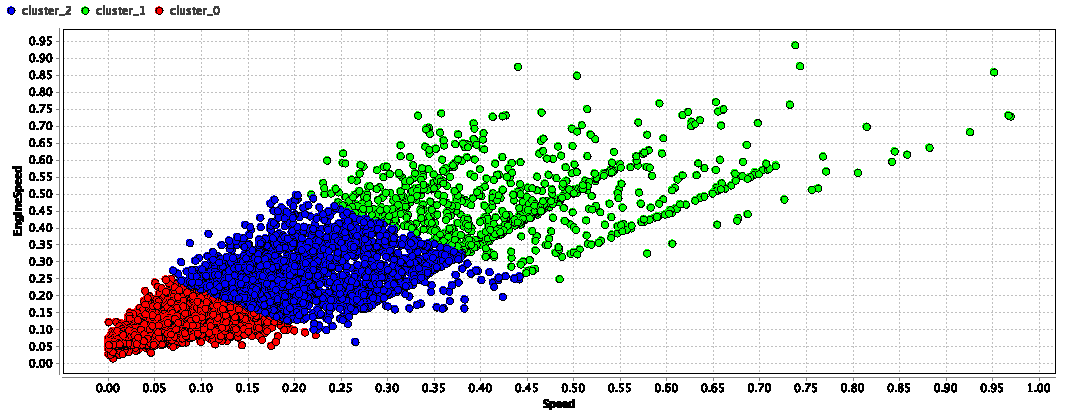
\includegraphics[width=\textwidth]{images/cluster_distrib.png}}
\caption{Clustering result}
\label{figure:clusters}
\end{figure}

From Figure~\ref{figure:clusters} we can easily deduce that \texttt{Speed} and \texttt{EngineSpeed} are correlated by means of a ``linear'' function. In fact Figure~\ref{figure:probedistspeed} and Figure~\ref{figure:probedistengspeed} which represents the distribution of \texttt{Probes} over clusters with respect to \texttt{Speed} and to \texttt{EngineSpeed} are very similar.

\begin{figure}[h!]
\centerline{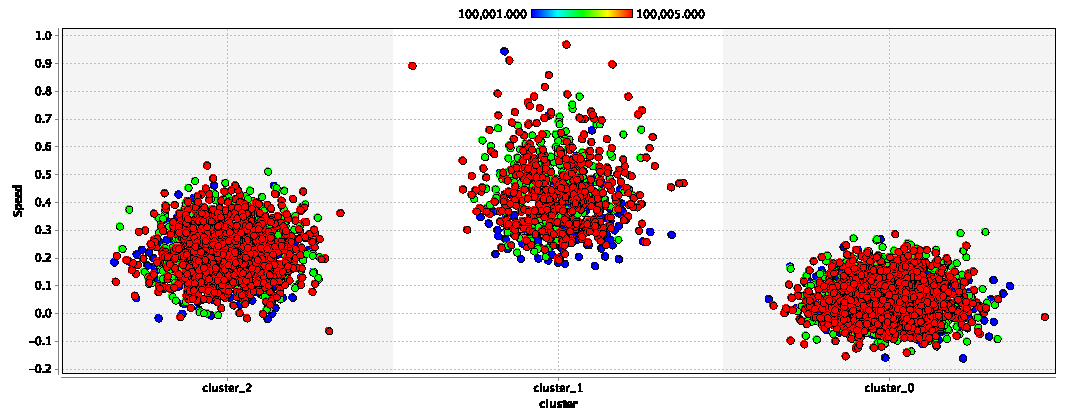
\includegraphics[width=\textwidth]{images/probe_cluster_distrib_speed.png}}
\caption{Probes distribution over clusters with respect to Speed}
\label{figure:probedistspeed}
\end{figure}

\begin{figure}[h!]
\centerline{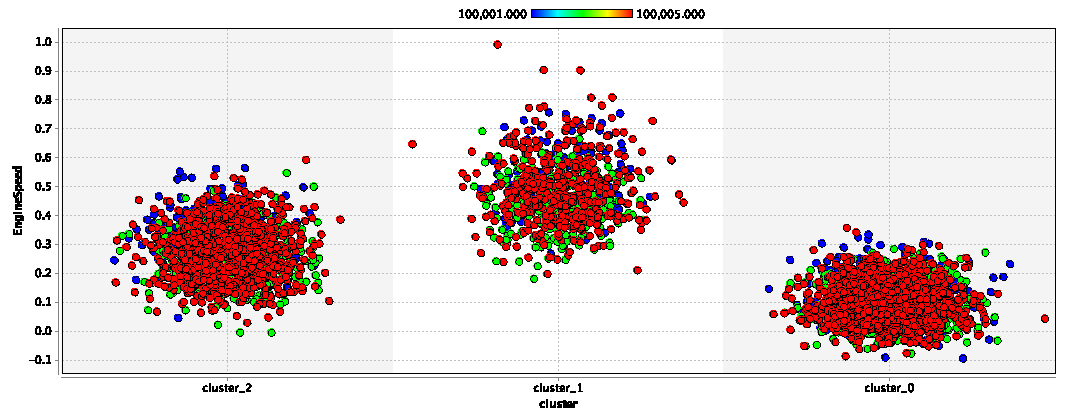
\includegraphics[width=\textwidth]{images/probe_cluster_distrib_enginespeed.png}}
\caption{Probes distribution over clusters with respect to EngineSpeed}
\label{figure:probedistengspeed}
\end{figure}

From both Figure~\ref{figure:probedistspeed} and Figure~\ref{figure:probedistengspeed} we can deduce that all vehicles assume all the three driving styles the mining process discovered.\\

Figure~\ref{figure:clustersdistribGPS} shows an interesting trend: clusters, which basically describe how a vehicle behaves, seems not to be correlated with GPS coordinates hence with the portion of the city in which the vehicle moves since all clusters are distributed over the cartesian graph.

\begin{figure}[h!]
\centerline{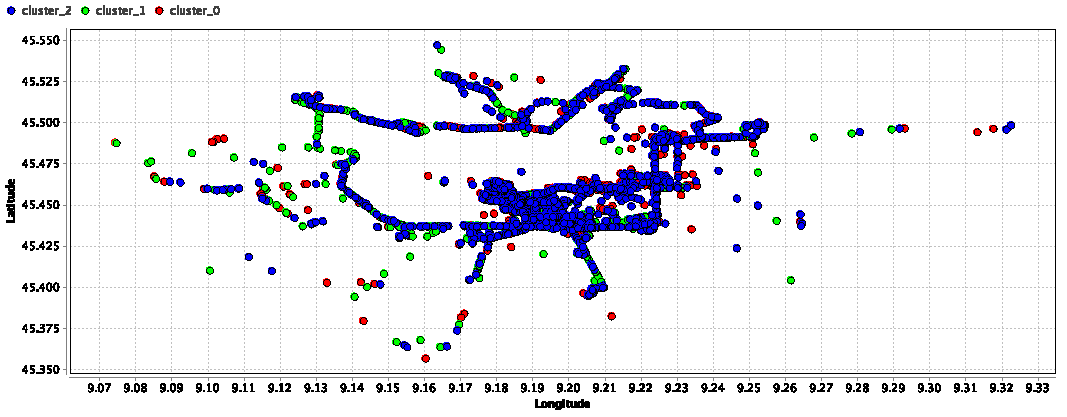
\includegraphics[width=\textwidth]{images/cluster_distrib_long_lat.png}}
\caption{Cluster distribution over GPS coordinates}
\label{figure:clustersdistribGPS}
\end{figure}

More information on this trend can be extracted from Figure~\ref{figure:speeddistribGPS1}, \ref{figure:speeddistribGPS3}, and \ref{figure:speeddistribGPS5} which are related to the three vehicles we analyzed.

\begin{figure}[h!]
\centerline{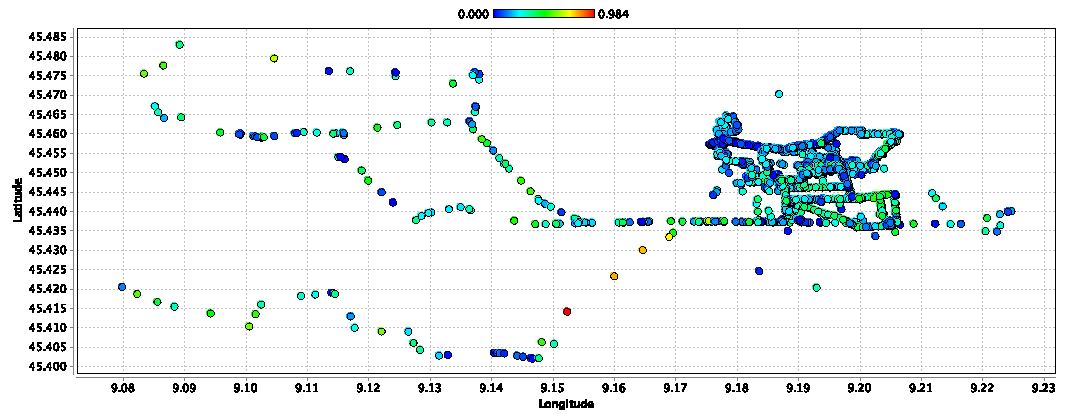
\includegraphics[width=\textwidth]{images/1_speed_distrib.png}}
\caption{Speed distribution over GPS coordinates}
\label{figure:speeddistribGPS1}
\end{figure}

\begin{figure}[h!]
\centerline{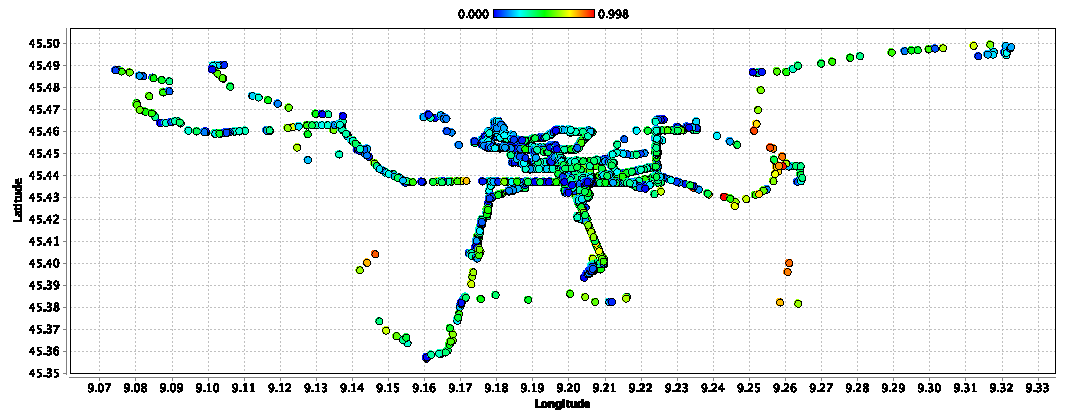
\includegraphics[width=\textwidth]{images/3_speed_distrib.png}}
\caption{Speed distribution over GPS coordinates}
\label{figure:speeddistribGPS3}
\end{figure}

\begin{figure}[t]
\centerline{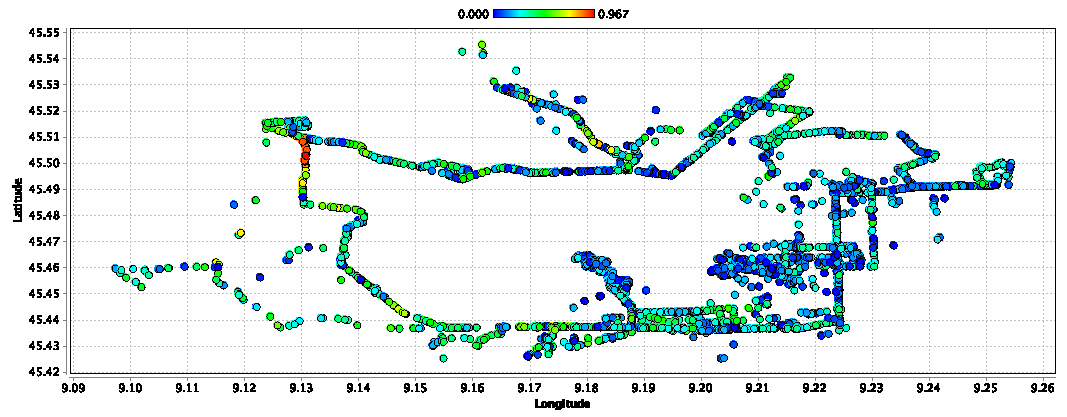
\includegraphics[width=\textwidth]{images/5_speed_distrib.png}}
\caption{Speed distribution over GPS coordinates}
\label{figure:speeddistribGPS5}
\end{figure}
